\documentclass{amsproc}
\usepackage{indentfirst}
\usepackage{amsthm}
\usepackage{amsmath}
\usepackage{amsfonts}
\usepackage{amssymb}
\usepackage{hyperref}
\usepackage{url}
\usepackage{tabto}
\usepackage{fancyvrb}
\usepackage{setspace}

\usepackage{caption}
\usepackage{subcaption}

\usepackage{graphicx}


\usepackage[noend]{algpseudocode}
\usepackage{algorithm}

\makeatletter
\def\BState{\State\hskip-\ALG@thistlm}
\makeatother

\setcounter{tocdepth}{2}

\title{The Fourier Transform: Variations and Applications}

\author{Sailesh Kaveti}

\renewcommand{\baselinestretch}{1.25}

\begin{document}

\maketitle


\tableofcontents
\newpage

\section{Complex Analysis Fundamentals}

\subsection{Basic Properties of Complex Numbers}

\mbox{}	 \\
\indent Saff and Snider, in \textit{Fundamentals of Complex Analysis with Applications to Engineering and Science} introduce a \textbf{complex number} as an expression in the form $a + bi$, where $a$ and $b$ must be real numbers and $i = \sqrt{-1}$. Two complex numbers $a +bi$ and $c + di$ can only be equal if and only if $a = c$ and $b = d$. For future reference, complex numbers will be referred to as $z$ where $z = a+bi$. A complex number $a+bi$ exists on the complex plane as a rectangular coordinate $(a, b)$. The following properties of complex numbers will be used over the course of this paper:

\begin{enumerate}
	\item $z = a+bi$
	\item $\bar{z} = a - bi$
	\item $|z| = \sqrt{a^2 + b^2}$
	\item $\overline{(z_1 z_2)} = \bar{z_1}\bar{z_2}$
	\item $Re(z) = a = \frac{z + \bar{z}}{2}$
	\item $Im(z) = b = \frac{z - \bar{z}}{2i}$
	\item $z \bar{z} = |z|^2$
	\item $|z_1 + z_2| \leq |z_1| + |z_2|$
\end{enumerate}

A complex number with rectangular coordinates $(x, y)$ can be written in terms of the polar coordinates $(r, \theta)$ such that

$$
x = rcos(\theta) \qquad y = rsin(\theta)
$$
Conversely, a polar coordinate can be written in terms of rectangular coordinates such that 
$$
r = \sqrt{x^2 + y^2} = |z| \qquad 
tan(\theta) = y/x
$$
It is important to note that 
$$
\theta = tan^{-1}\Big(\frac{y}{x}\Big)
$$
does not necessarily hold true because $\theta$ can exist in different quadrants while $tan(\theta)$ still has the same value.

\subsection{Roots of Unity}

\mbox{}	 \\
\indent Before starting the Fast Fourier Transform (FFT), it is important to introduce a concept known as complex roots of unity. A complex $n^{th}$ root of unity is a complex number $\omega$ such that $\omega^n = 1$. As the name suggests, there are a total of $n$ distinct complex $n^{th}$ roots of unity. In order to find all $n$ complex roots of unity, we say $\omega_k = e^{\frac{2 \pi i k}{n}}, \forall k \in \{0, 1, 2, ... , n-1\}$. When $k = 0$, we yield the trivial solution of $\omega = 1$.

\subsection{Euler's Formula}

\mbox{}	 \\
\indent In this subsection, we explore the relationship between the mathematical constant $e$ and the trigonometric functions $cosine$ and $sine$ as well as the imaginary constant $i$. Let $z = x + iy$.

\begin{align*}
z &= x + iy \\
e^{z} &= e^{x+iy} \\
&= e^x e^{iy}
\intertext{We can then differentiate the second term on the right hand side to determine that}
\frac{de^{iy}}{d(iy)} &= e^{iy} \\
\frac{de^{iy}}{dy} &= ie^{iy}
\intertext{Differentiating again, we get: }
\frac{d^2e^{iy}}{dy^2} &= \frac{d}{dy}(ie^{iy}) \\
&= i^2 e^{iy} \\
&= -e^{iy}
\intertext{We are left with the following differential equation, that if}
g(y) &= e^{iy}
\intertext{then, }
\frac{d^2g}{dy^2} &= -g
\intertext{and that any function in the form of }
g(y) &= Acos(y) + B sin(y)
\intertext{satisfies the differential equation. To evaluage A and B, we can use the following equations: }
g(0) &= e^{i0} = 1 = A cos(0) + B sin(0) \\
\frac{dg}{dy}(0) &= ie^{i0} = i = -Asin(0) +Bcos(0)
\intertext{Thus, }
& \quad \quad A = 1 \quad \quad B = i
\intertext{and}
e^{iy} &= cos(y) + i sin(y)
\end{align*}
Thus, \textbf{Euler's Formula} is as follows:
$$
e^{i\theta} = cos(\theta) + i sin(\theta)
$$


\section{The Fourier Transform}

\subsection{Developing an Intuition for the Fourier Transform}

\mbox{}	\\
\indent Imagine we are given we are given a bucket of paint, and asked to replicate the color of that bucket. At first, it seems easy to simply describe it nominally, calling the bucket of paint as red, yellow, blue, or any other color.  This is a valid first instinct. However, imagine you were given a purple bucket of paint. Even in this instance, most people are familiar with the color purple and we could just mix equal parts of blue and red. Imagine you were given a bucket of paint that was dark purple. We could still call this bucket “dark purple”, but we would immediately run into problems when replicating the paint color. Do we need to put the colors on a 2:1 ratio or a 3:1 ratio? In general, given a color, it can be very useful to know the colors that compose that color, as opposed to just a nominal description. Now imagine that we were given a complex wave, and that we are interested in the simpler waves that compose that wave. The Fourier Transform helps us determine a periodic wave's composite frequencies.

\subsection{The Fourier Series}

\mbox{}	\\
\indent In order to understand the Fourier Transform, it is very important to gain understand the Fourier Series and its integral and the Fourier Transform is non-discretized extension of the Fourier Series. According to Dym and McKean, the authors of \textit{Fourier Series and Integrals}, the basic idea of the Fourier Series is that any periodic function $f(t)$ can be expressed as a trigonometric sum of sines and cosines. More specifically, for the same period T for both $sine$ and $cosine$, we can claim the following:

$$
f(t) = \sum_{n = 0}^{\infty} [\hat f_+(n)\cos \Big(\frac{\pi n t}{T}\Big) + \hat f_-(n)\sin \Big(\frac{\pi n t}{T}\Big)]
$$

From this, we can derive the equations for $\hat f_+(n)$ and $\hat f_-(n)$. The equations are as follows

\begin{align*}
\hat f_+(n)  &= \frac{1}{L}\int_{-L}^{L} f(t) cos\Big(\frac{n\pi x}{L}\Big)dx \\
\hat f_-(n)  &= \frac{1}{L}\int_{-L}^{L} f(t) sin\Big(\frac{n\pi x}{L}\Big)dx
\end{align*}

Putting these two together, we can get the Fourier Series, a formula to completely put a periodic function in terms of $sine$ and $cosine$. For example, a non-analytic square wave $g(x)$, that has a value of $-h$ from $-\pi$ to $0$ and h from $0$ to $pi$ with a vertical line from $-h$ to $h$ can be modeled with the following Fourier Series:

$$
g(x) = \sum_{n = 0}^{\infty} \frac{sin((2n + 1)x)}{(2n + 1)}
$$

The intuition behind a Fourier Series is very similar to a Taylor or MacLaurin Series, where a complex function can be modeled and very closely  as an infinite sum of simpler functions.

\subsection{The Computation of the Fourier Transform}

\mbox{}	\\
\indent Similar to colors, given a complex wave, it is important to know the frequencies that compose that wave. The inverse of this can also provide us with valuable information. A wave $f(x)$ exists in real space, and its equivalent in frequency space is function $F(s)$. In short, $f(x)$ gives us a complex wave in real space, while $F(s)$ gives us a function with peaks at the frequencies that make up $f(x)$.

As described in \textit{The Fourier Transforms and Its Applications}, the following relationship between F(s) and f(x) exists:
\begin{align*}
\intertext{The Fourier Transform:}
F(s)  &= \int_{-\infty}^{\infty} f(x) e^{-i2 \pi x s}dx
\intertext{The Inverse Fourier Transform:}
f(x)  &= \int_{-\infty}^{\infty} F(s) e^{i2 \pi x s}ds
\end{align*}

Replacing any instances of $e^{i\theta}$ with $cos(\theta) + isin(\theta)$, we can derive the following equivalent expressions:
\begin{align*}
\intertext{The Fourier Transform:}
F(s)  &= \int_{-\infty}^{\infty} f(x) (cos(-2 \pi x s) + isin(-2 \pi x s))dx
\intertext{The Inverse Fourier Transform:}
f(x)  &= \int_{-\infty}^{\infty} F(s) (cos(2 \pi x s) + isin(2 \pi x s))ds
\end{align*}

As a result, we can see a resemblance of a non-discretized version of the Fourier Series, which we can discretize for more interesting results in the following section.

\section{The Discrete Fourier Transform}

\subsection{The Basics of the Discrete Fourier Transform}

\mbox{}	 \\
\indent As the name suggests, the Discrete Fourier Transform (DFT) is a discretized, more applicable version of the regular Fourier Transform. According to Gonzalez and Woods, the authors of \textit{Digital Image Processing}, the DFT is a derivation of the Fourier Transform and the Inverse DFT is a derivation of the Inverse Fourier Transform. The derivation for the DFT and IDFT are not included, but involve sampling a finite number of points from the Fourier Transforms.

\begin{align*}
\intertext{The Fourier Transform:}
F(s)  &= \int_{-\infty}^{\infty} f(x) e^{-i2 \pi x s}dx
\intertext{The Discrete Fourier Transform:}
F(s) &= \frac{1}{N} \sum_{x=0}^{N-1} f(x) e^{-i2 \pi x s / N}
\intertext{The Inverse Fourier Transform:}
f(x)  &= \int_{-\infty}^{\infty} F(s) e^{i2 \pi x s}ds
\intertext{The Inverse Discrete Fourier Transform}
f(x) &= \sum_{s=0}^{N-1} F(s) e^{-i2 \pi x s / N}
\end{align*}

In \textit{The Discrete Fourier Transform}, Sundararajan claims that the DFT is able to transform a $N$-point time-domain sequence into a set of $N$ frequency coefficients that represent the given time-domain sequence in frequency domain. These coefficients represent magnitudes and the amplitudes of the composite $sine$ and $cosine$ counterparts. When these composite functions are added, the original time-domain sequence is represented. However, we are presented with a strange dilemma. It doesn't seem intuitive to represent a finite length sequence with a sum of infinite sinusoidal waves. However, any finite length sequence that is the sum of sinusoidal waves must be periodic, and thus can be extended periodically. On the other hand, the IDFT can transform the $N$ frequency coefficients back into the original set of $N$ time-domain samples but creating a composition of the sinusoidal waves to generate the original signal. Thus, every signal has two characterizations: its $N$ time-domain samples or its $N$ frequency coefficients.

There are also several interesting properties of the Discrete Fourier Transformation that hold true that allow for more informative results. An example of such a property is known as \textbf{Parseval's Theorem}. This theorem implies that the sums of the squared magnitudes of the signal and the DFT sequences are directly related by the constant $N$, which has already been established as the number of samples. Mathematically, we can write that

$$
\sum_{n=0}^{N-1} |x(n)|^2 = \frac{1}{N} \sum_{k=0}^{N-1} |X(k)|^2
$$

Sundararajan explains the proof as the following:
\begin{align*}
\intertext{Since the square of the magnitude of a complex number can be written in terms of its and its conjugate, the following holds true:}
\sum_{n=0}^{N-1} |x(n)|^2 &= \sum_{n=0}^{N-1} x(n) x^{*}(n)
\intertext{Substituting the corresponding IDFT expressions for both x(n) and its conjugate, we can get}
&= \sum_{n=0}^{N-1} \frac{1}{N^2} \sum_{k=0}^{N-1} \sum_{m=0}^{N-1} X(k)X^{*}(m)W_{N}^{-n(k-m)} \\
&= \frac{1}{N^2} \sum_{k=0}^{N-1} \sum_{m=0}^{N-1} X(k)X^{*}(m) \sum_{n=0}^{N-1} W_{N}^{-n(k-m)} \\
\intertext{When k = m, this expression can be simplified to}
&= \frac{1}{N} \sum_{k=0}^{N-1} X(k) X^{*}(k) \\
&= \frac{1}{N} \sum_{k=0}^{N-1} |X(k)|^2 
\intertext{When this does not hold true, the equation reduced to zero because of the orthogonal property}
\end{align*}

\section{The Computation of the Discrete Fourier Transform}

\subsection{The Fast Fourier Tranform}


\mbox{}	 \\
\indent Given the Discrete Fourier Transform, it seems in our interest to find a way to compute this value. In \textit{Introduction to Algorithms}, Cormen, Leiserson, Rivest, and Stein introduce the FFT which they claim takes advantage of of the special properties of the complex roots of unity to compute $DFT_n(a)$ in $O(nlog(n))$. For the sake of this implementation, they assume at $n$ is a power of two, mostly because the existing strategies for dealing with the case where $n$ is not a power of two are quite complex. As the runtime of the algorithm suggests, the FFT is a divide and conquer algorithm. Given an $A(x)$, we can represent it as an array $a$ of coefficients. In addition, we must also define the following intermediary functions that will be called in the algorithm:
	
\begin{align*}
A^{[0]}(x) &= a_0 + a_2x + a_4x^2 + ... + a_{n-2}x^{n/2 - 1} \\
A^{[1]}(x) &= a_1 + a_3x + a_5x^2 + ... + a_{n-1}x^{n/2 - 1} \\
\intertext{such that}
A(x) &= A^{[0]}(x^2) + xA^{[1]}(x^2)
\end{align*}

The following algorithm to find the FFT of $a$ is defined recursively by Cormen and is as follows:

\begin{algorithm}
\caption{Recursive Implementation of FFT}\label{fft}
\begin{algorithmic}[1]
\Procedure{Recursive-FFT}{a} \Comment{A Recursive Implementation of FFT}
\State $n = a.length$
\If {$n == 1$} \Return{ a} \Comment{Base Case of Recursion}
\EndIf
\State $\omega_n = e^{2\pi i / n}$ 
\State $\omega = 1$
\State $a^{[0]} = (a_0, a_2, a_4, ..., a_{n-2})$ \Comment{Define Coefficients}
\State $a^{[1]} = (a_1, a_3, a_5, ..., a_{n-1})$
\State $y^{[0]} = \Call{Recursive-FFT}{a^{[0]}}$ \Comment{Recursive Step}
\State $y^{[1]} = \Call{Recursive-FFT}{a^{[1]}}$

\For{ \texttt{$k = 0$ to $n/2 - 1$}}
	\State $y_k = y_k^{[0]} + \omega y_k^{[1]}$ \Comment{These hold true by definition of $y_k$}
	\State $y_{k+(n/2)} = y_k^{[0]} - \omega y_k^{[1]}$
	\State $\omega = \omega \omega_n$ \Comment{Making sure that $\omega$ is updated properly}
\EndFor

\State \Return{y} \Comment{Assumed that $y$ is a column vector}

\EndProcedure
\end{algorithmic}
\end{algorithm}

From this algorithm, we can arrive at the \textbf{Convolution Theorem}, which states that for any two vectors $a$ and $b$, both of which have a length $n$ that is a power of two, the following holds true:

$$
a \otimes b = DFT_{2n}^{-1}(DFT_{2n}(a) DFT_{2n}(b))
$$

\subsection{Alternatives for the Fast Fourier Tranform}

\mbox{}	 \\
\indent In \textit{Introduction to Algorithms}, Cormen, Leiserson, Rivest, and Stein present certain improvements to existing implementation of the FFT. One notable improvement is an iterative implementation of the FFT. In Computer Science, iterative and recursive solutions are often considered equivalent. This is proved in the Church-Turing Thesis. However, there certainly runtime tradeoffs that we sometimes have to make when converting from recursion to iteration and vice-versa. That being said, we make no computational trade-offs in this instance, as our iterative solution still has a runtime of $O(nlog(n))$. In this instance, just like the recursive implementation, $a$ must have a length that is a power of 2. The algorithm for an iterative approach to the FFT is as follows:

\begin{algorithm}
\caption{Iterative Implementation of FFT}\label{it-fft}
\begin{algorithmic}[1]
\Procedure{Bit-Reverse-Copy}{a, A} 

\State $n = a.length$
\For {\texttt{$k = 0$ to $n-1$}}
	\State $A[rev(k)] = a_k$ \Comment{$rev(k)$ is the reverse of the bit-wise representation of k}
\EndFor

\EndProcedure

\Procedure{Iterative-FFT}{a}

\State \Call{Bit-Reverse-Copy}{a, A}
\For {\texttt{$s = 1$ to $log_2(n)$}}
	\State $m = 2^s$
	\State $\omega_m = e^{2 \pi i / m}$
	\For {\texttt{$k = 0$ to $n - 1$ by $m$}}
		\State $w = 1$
		\For {\texttt{$j = 0$ to $m/2 - 1$}}
			\State $t = \omega A[k + j + m/2]$
			\State $u = A[k+j]$
			\State $A[k+j] = u + t$
			\State $A[k+j+m/2] = u - t$
			\State $\omega = \omega \omega_m$
		\EndFor
	\EndFor
\EndFor

\EndProcedure

\end{algorithmic}
\end{algorithm}

\subsection{A Python Implementation of the Fast Fourier Transform}

\mbox{}	 \\
\indent In order to better understand the results of the Fast Fourier Transform, it may be useful to write code to explore a Pythonic implementation, and  plot the signals in order to visualize the results of the Fast Fourier Transform. There are existing libraries in Python to aid with the visualization of the Fast Fourier Transformation. These include numpy and matplotlib. Numpy is useful for existing libraries that make it possible to manipulate an entire array with a single operation as well as contains the function to perform the Fast Fourier Transformation. Matplotlib is the library that contains the function to fully plot a dataset. Given a signal, the following method plots both the signal in real space as well as in frequency space:

\begin{Verbatim}[tabsize=4]

def plot_signal(signal):
	signal_fft = np.fft.fft(signal)
	signal_fft_pow = np.abs(signal_fft)
	plt.plot(signal, '-o', markersize = 2)
	plt.savefig('RealSpace.png')
	plt.clf()
	plt.plot(signal_fft_pow, '-o', markersize = 2)
	plt.savefig('FrequencySpace.png')
	
\end{Verbatim}

With that information, we are able to quickly find the FFT of different waves in real space in frequency space. Here are a few examples generated as a result of the python code included above. 

\begin{figure}[h]
\centering
\begin{subfigure}{.4\textwidth}
	\centering
	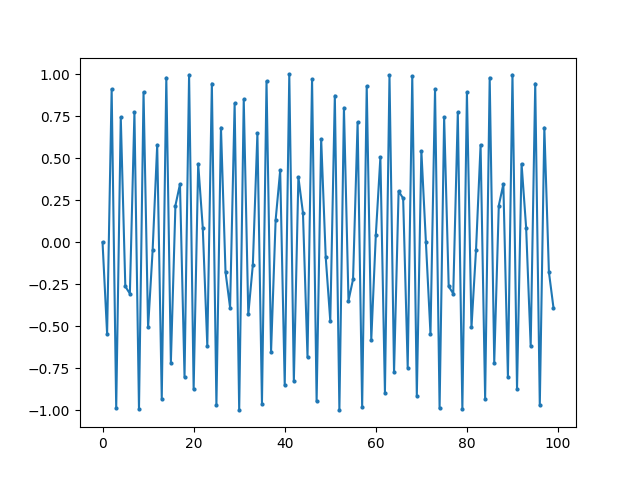
\includegraphics[scale=.3]{images/FFTOriginal1.png}
	\caption{Real Space}
	\label{fig:sub1}
\end{subfigure} %
\begin{subfigure}{.4\textwidth}
	\centering
	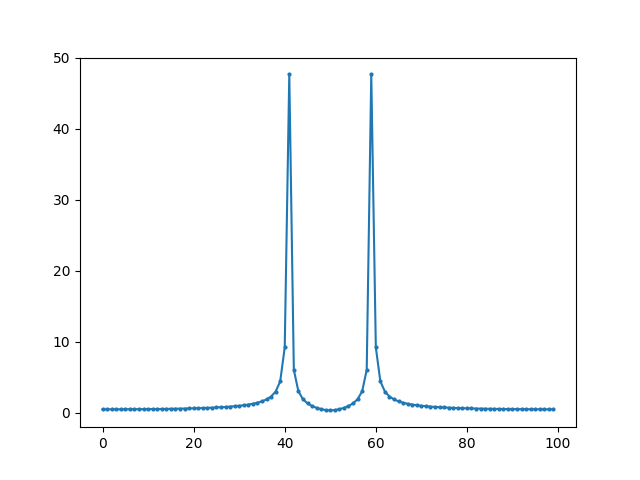
\includegraphics[scale=.3]{images/FFTResult1.png}
	\caption{Frequency Space}
	\label{fig:sub2}
\end{subfigure}
\caption{Wave 1 and its Fast Fourier Transform}
\label{fig:text1}
\end{figure}


\begin{figure}[h]
\centering
\begin{subfigure}{.4\textwidth}
	\centering
	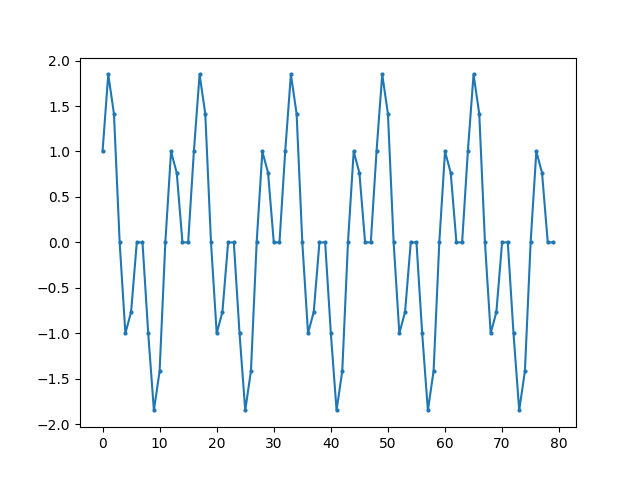
\includegraphics[scale=.3]{images/FFTOriginal2.png}
	\caption{Real Space}
	\label{fig:sub3}
\end{subfigure} %
\begin{subfigure}{.4\textwidth}
	\centering
	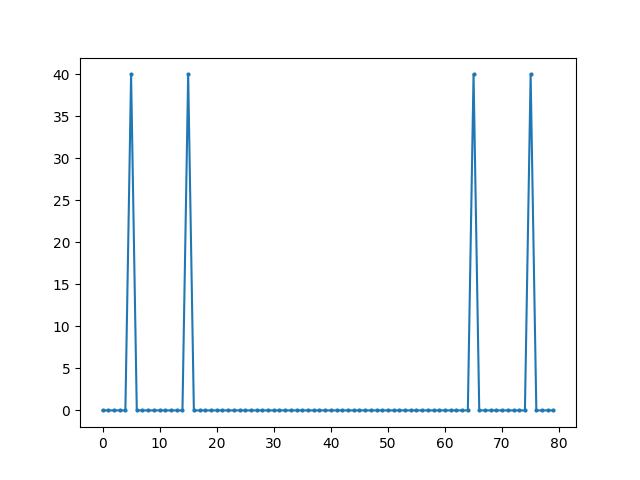
\includegraphics[scale=.3]{images/FFTResult2.png}
	\caption{Frequency Space}
	\label{fig:sub4}
\end{subfigure}
\caption{Wave 2 and its Fast Fourier Transform}
\label{fig:text2}
\end{figure}

\begin{figure}[h]
\centering
\begin{subfigure}{.4\textwidth}
	\centering
	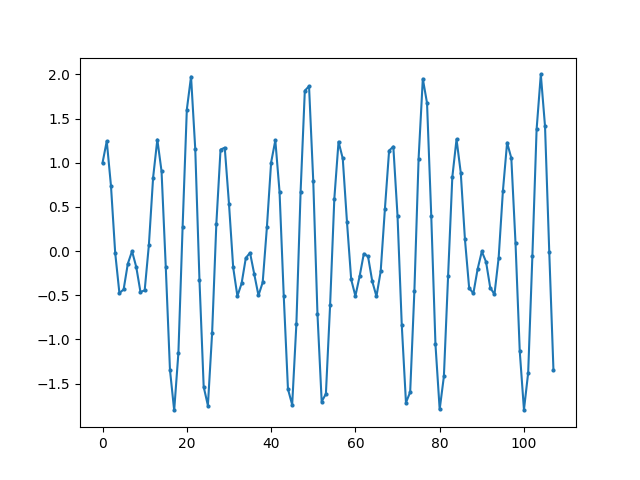
\includegraphics[scale=.3]{images/FFTOriginal3.png}
	\caption{Real Space}
	\label{fig:sub3}
\end{subfigure} %
\begin{subfigure}{.4\textwidth}
	\centering
	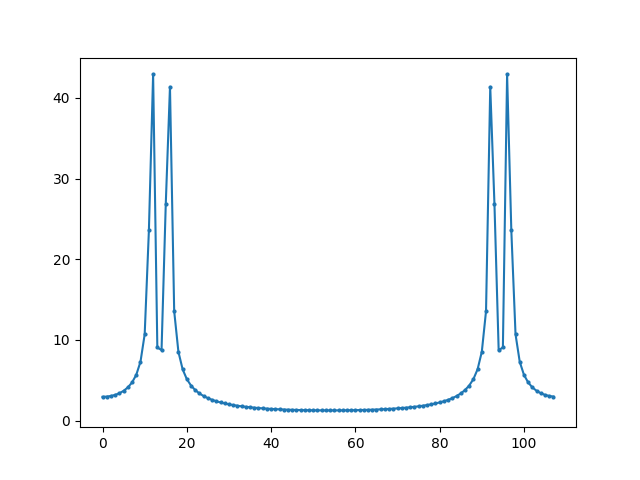
\includegraphics[scale=.3]{images/FFTResult3.png}
	\caption{Frequency Space}
	\label{fig:sub4}
\end{subfigure}
\caption{Wave 3 and its Fast Fourier Transform}
\label{fig:text3}
\end{figure}
\section{Applications of the Fourier Transform}

\subsection{Multiplication of Polynomials}

\mbox{}	 \\
\indent According to \textit{Introduction to Algorithms}, the straightforward method of adding two polynomials takes $O(n)$ time. We know the following to hold true:

\begin{align}
f(x) &= \sum_{j = 0}^{n} a_j x^j \\
g(x) &= \sum_{j = 0}^{n} b_j x^j \\ 
f(x) + g(x) &= \sum_{j = 0}^{n} (a_j + b_j)  x^j 
\end{align}

For two polynomials $f(x)$ and $g(x)$, with length $k$ and $n$, we know that $f(x) + g(x)$ has length $max(k, n)$. Generate two arrays of length $n$ called $A_f$ and $A_g$ where each index $i$ represents the coefficient for term $x^i$ for $f(x)$ and $g(x)$ respectively. Iterate through the arrays and add the value held at each index of $A_f[i]$ and $A_g[i]$ and set that value in $A_{f+g}[i]$. The resulting array represents the coefficients of $f(x)+g(x)$.

With this in mind, we can derive the straightforward algorithm for the multiplication of two polynomials. For the multiplication of the two polynomials, Cormen claims that the following holds true:

\begin{align}
f(x)g(x) &= \sum_{j = 0}^{2n} c_j  x^j \\
\intertext{where}
c_j &=  \sum_{k = 0}^{j} a_k b_{j-k}
\end{align}

From this information, we can see that equation $(4)$ yields us with the sum of $2n$ polynomials, each of which was computed in $O(n)$ time. As we showed earlier, the sum of any two polynomials can be computed in $O(n)$ time, and since we must add $2n$ total polynomials, we get that the product of any two polynomials can be computed in $O(2n^2)$ time, which can be reduced to $O(n^2)$ time by the definition of big-$O$ notation.

With our understanding of the FFT, Cormen claims that we can find the product of any two polynomials in $O(nlog(n))$ time, a significant asymptotic improvement over $O(n^2)$.  Before starting the explanation of the algorithm, it is important to introduce another way to represent a polynomial, known as the point-value representation. 

The point-value representation of a polynomial $A(x)$ is a set of pairs in the form ${\{(x_0, y_0), (x_1, y_1), ..... , (x_n, y_n)\}}$ such that $y_i = A(x_i)$.  These values can be generated in $O(n^2)$  time using Horner's Metho, but can be reduced to $O(nlog(n))$ time if the values of $x$ are cleverly picked. From this definition, one can conclude that each polynomial has a many different point-value representations. Using this new representation of polynomials, we can indeed determine the product of any two polynomials in $O(n)$ time. Given this information, we can now explore the algorithm to find the product of any two polynomials in $O(nlog(n))$ time. Cormen argues that the following four steps will determine the product of any two polynomials $A(x)$ and $B(x)$ of length n:

\begin{enumerate}
	\item \textit{Double degree-bound: } Create the coefficient representations of $A(x)$ and $B(x)$ of length $2n$ by padding $n$ higher-order coefficients to the left of the array representations of $A(x)$ and $B(x)$. This can be done in $O(n)$ time.
	\item \textit{Evaluate: } Compute the point-value representations of $A(x)$ and $B(x)$ of length $2n$ by applying the FFT of order $2n$ on each polynomial. As a result, we can get the representations at the $(2n)^{th}$ roots of unity. This is done in $O(nlog(n))$ time.
	\item \textit{Pointwise Multiply: } Multiply these two point-value representations pairwise, yielding us with the value of $C(x) = A(x)B(x)$ at all roots of unity. As explained earlier, this is done in $O(n)$ time.
	\item \textit{Iterpolate: } We can then create the coefficient representation of polynomial  $C(x)$ by applying the FFT on the point-value representation of $C(x)$. This is done in $O(nlog(n))$ time.

\end{enumerate}

This entire process is done in $O(n + nlog(n) + n + nlog(n))$ time, which can reduce to $O(nlog(n))$ time by the definition of big-$O$ notation. Thus, using the above algorithm, one can multiply any two polynomials in $O(nlog(n))$ time.

\subsection{Image Processing}

\mbox{}	 \\
\indent According to Gonzalez, ``an image may be defined as a two-dimensional function, $f(x, y)$ where $x$ and $y$ are \textit{spatial} (plane) coordinates, and the amplitude of $f$ at any pair of coordinates $(x, y)$ is called the \textit{intensity} or \textit{gray level} of the image at that point''. In short, an image can be represented by a function that determines the color at a certain pixel. Digital image processing is one of the most widespread fields of study, having applications in virtually every STEM related profession. In addition, digital imaging processing is also not bound to visible light spectrum. We can perform image processing is the Gamma spectrum, X-ray spectrum as well as the Ultraviolet Band. Included are a few examples of imaging outside the visible light spectrum.

\begin{figure}[h]
\centering
\begin{subfigure}{.3\textwidth}
	\centering
	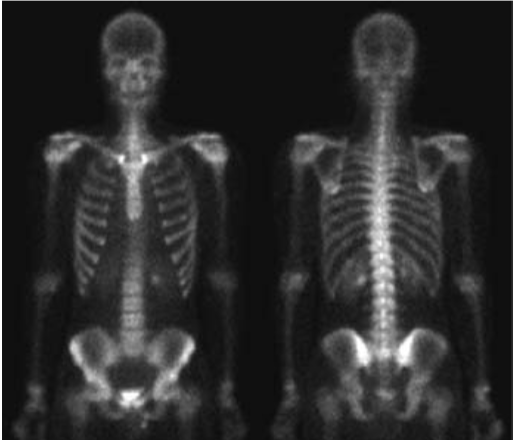
\includegraphics[scale=.25]{images/gamma.png}
	\caption{Gamma-Ray Imaging}
	\label{fig:sub5}
\end{subfigure} %
\begin{subfigure}{.3\textwidth}
	\centering
	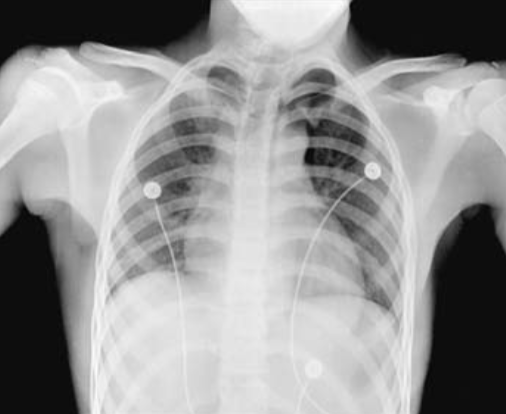
\includegraphics[scale=.25]{images/xray.png}
	\caption{X-Ray Imaging}
	\label{fig:sub6}
\end{subfigure} %
\begin{subfigure}{.3\textwidth}
	\centering
	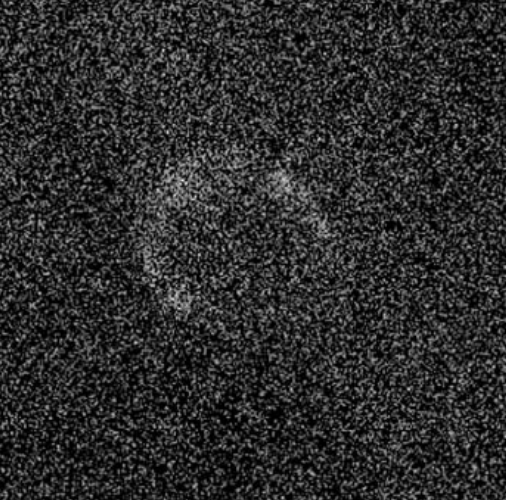
\includegraphics[scale=.25]{images/uv.png}
	\caption{Ultraviolet Imaging}
	\label{fig:sub7}
\end{subfigure}
\caption{Imaging across various sources}
\label{fig:im1}
\end{figure}

In every variation of the Fourier Transform above, we were working in one dimension. If we were to follow a similar derivation described above, we can indeed arrive as a two-dimensional DFT and a two-dimensional IDFT. 
\begin{align*}
\intertext{Two-Dimensional Discrete Fourier Transform}
F(u, v) &= \sum_{x=0}^{M-1}\sum_{y=0}^{N-1} f(x, y) e^{-i2\pi (ux/M + vy/N)}
\intertext{Two-Dimensional Inverse Discrete Fourier Transform}
f(x, y) &= \frac{1}{MN}\sum_{x=0}^{M-1}\sum_{y=0}^{N-1} F(u, v) e^{i2\pi (ux/M + vy/N)}
\end{align*}
In this case, $f(x, y)$ is a digital image of size $M \times N$, and just like in the 1-D case, must be evaluated for the discrete values $u$ and $v$ in the ranges $u = 0, 1, 2, ..., M-1$ and $v = 0, 1, 2, ... , N-1$

The two-dimensional DFT is an essential part of modern image processing and is essential in various aliasing and filtering techniques. For example, Gonzalez includes following application of the Discrete Fourier Transform:


\begin{figure}[h]
\centering
\begin{subfigure}{.3\textwidth}
	\centering
	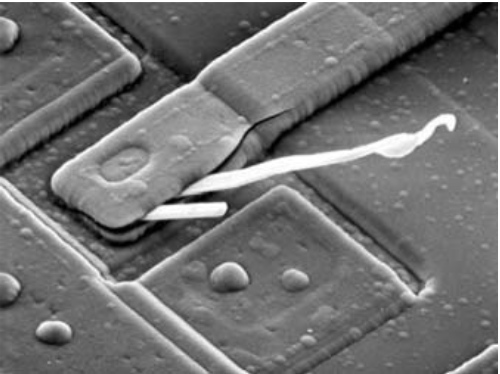
\includegraphics[scale=.32]{images/dftimage1.png}
	\caption{A Damaged Circuit}
	\label{fig:sub8}
\end{subfigure} %
\begin{subfigure}{.3\textwidth}
	\centering
	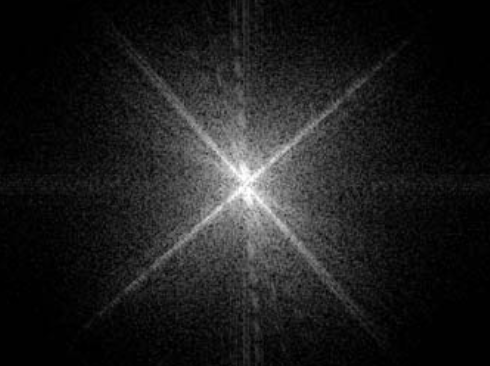
\includegraphics[scale=.32]{images/dftimage2.png}
	\caption{DFT on the Circuit}
	\label{fig:sub9}
\end{subfigure} %
\begin{subfigure}{.3\textwidth}
	\centering
	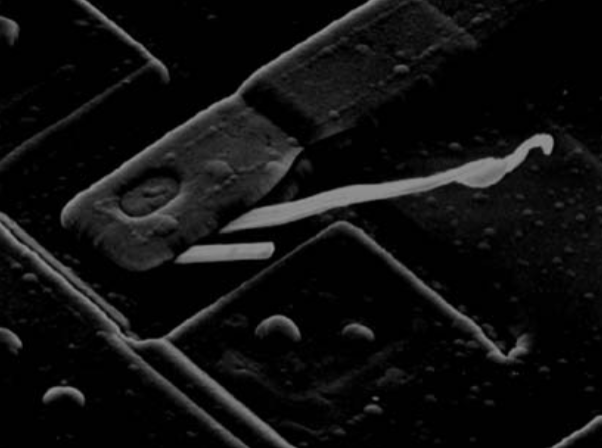
\includegraphics[scale=.25]{images/dftimage3.png}
	\caption{Modified IDFT (Dark)}
	\label{fig:sub10}
\end{subfigure}
\caption{Results of DFT and IDFT}
\label{fig:im2}
\end{figure}

In order to better explain the two-dimensional Discrete Fourier Transform, it may help to suggest a Python implementation for the algorithm to automate the conversion between an image and its Fourier Transform. Just like the one-dimensional Fast Fourier Transform, there are multiple existing tools and libraries to aid with the visualization of the two-dimensional Discrete Fourier Transform. Like the implementation of the 1-D FFT, the method to visualize the 2-D DFT involved numpy and matplotlib. In order to generate images, the 2-D DFT method also involves a library known as Pillow/PIL. Given an image, the following method displays the image as well as it's 2-D Discrete Fourier Transform:

\begin{Verbatim}[tabsize=4]

def plot_2d_dft(image):
	img = Image.open(image)
	img_arr = np.asarray(img)
	fourier = np.fft.fft2(img_arr)
	fourier = np.fft.fftshift(fourier)
	
	fourier = np.abs(fourier)
	fourier = fourier + 0.0000001
	fourier = np.log10(fourier)
	
	lowest = np.nanmin(fourier[np.isfinite(fourier)])
	highest = np.nanmax(fourier[np.isfinite(fourier)])
	original_range = highest - lowest
	norm_fourier = (fourier - lowest) / original_range * 255
	fourier_img = Image.fromarray(norm_fourier.astype('uint8'))
	fourier_img.save('2ddft1.png')
	
\end{Verbatim}

With this method, we are able to generate the two-dimensional DFT for any black and white image. Here are a few examples of the method being run on the image on the left:

\begin{figure}[h]
\centering
\begin{subfigure}{.4\textwidth}
	\centering
	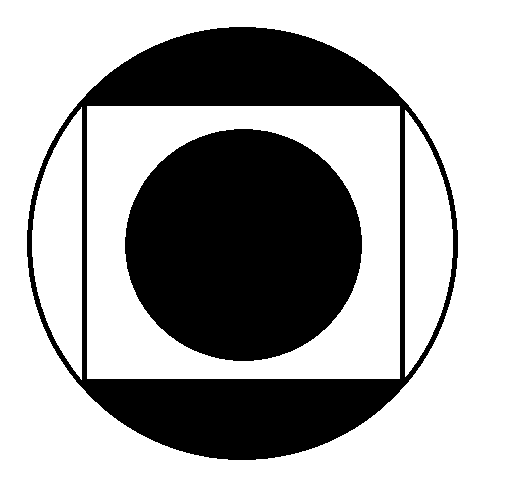
\includegraphics[scale=.3]{images/dftraw1.png}
	\caption{Original Image}
	\label{fig:sub11}
\end{subfigure} \hspace{15mm}
\begin{subfigure}{.4\textwidth}
	\centering
	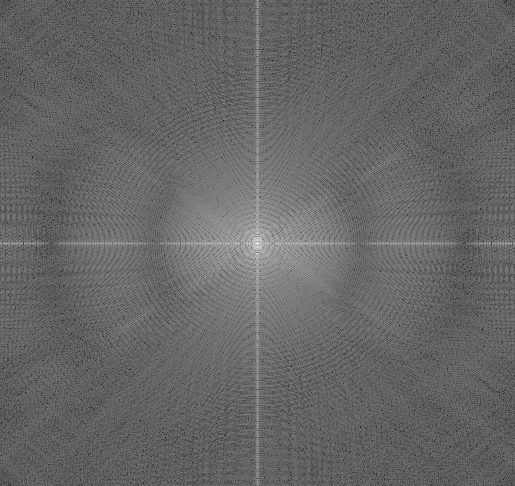
\includegraphics[scale=.3]{images/2ddft1.png}
	\caption{Fourier Transform}
	\label{fig:sub12}
\end{subfigure}
\caption{The Two-Dimensional DFT of Image 1}
\label{fig:im3}
\end{figure}

\begin{figure}[h]
\centering
\begin{subfigure}{.4\textwidth}
	\centering
	
\includegraphics[scale=.55]{images/circles.png}
	\caption{Original Image}
	\label{fig:sub11}
\end{subfigure} \hspace{15mm}
\begin{subfigure}{.4\textwidth}
	\centering
	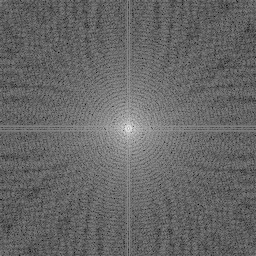
\includegraphics[scale=.6]{images/2ddft2.png}
	\caption{Fourier Transform}
	\label{fig:sub12}
\end{subfigure}
\caption{The Two-Dimensional DFT of Image 2}
\label{fig:im3}
\end{figure}

\subsection{Audio Compression}

\mbox{}	 \\
\indent Audio compression is an incredibly important field of study that attempts to address human and computer limitations on audio in order to effectively transmit information. In \textit{Audio Compression using Fourier Transform}, Perinati Tewari describes audio compression is the idea of encoding audio data to not only occupy less storage, but also less bandwidth for transmission. That being said, there are two conventional categories for compression, both of which are applicable for this algorithm: lossless and lossy compression. Tewari claims that lossless compression is done using various waveform coding techniques. What this means is that these techniques approximate the waveform with a more easily representable with a different sinusoidal function, and if the bit rate is large enough, get arbitrarily close to the original wave. A common technique is pulse code modulation (PCM), which is used by the CD. CD audio signals are conventionally samples at 44.1 kHz and traditionally add additional noise to the audio. However, this additional noise is not noticeable by the overwhelming majority of humans if the signal energy is large enough. In lossless compression, as highlighted, information is not lost. On the other hand, loss compression reduces redundancies  and any sounds that are considered irrelevant are either removes or significantly reduced.

With that information, it becomes easy to imagine why the Fourier Transform is important for Audio Compression. More specifically, the FFT can be applied to a audio signal to convert it to an approximate, much smaller signal. In addition, before beginning, Tewari states that most audio compression software makes use of the psycho-acoustic properties of the human auditory system. This is an important note given that audio compression algorithms are allows to make discretionary decisions because audio compression is always ``filtered'' through the human ear. 

Tewari proposes the following algorithm for using FFT to compress an audio signal:

\begin{enumerate}

	\item \textit{Level Detection: }The start of an input audio signal is identified by a stored threshold value
	\item \textit{Framing: }The continuous signal is blocked into frames of N samples. It is important to note that each frame overlaps with subsequent frames,  a technique known as framing.
	\item \textit{Windowing: }After framing, windowing is applied to prevent leakage. A windows is a shape that is nonzero for a certain period of time, and zero before and after that period. Thus, when a window is multiplied by a certain signal, it is zero everywhere except during of the nonzero period.
	\item \textit{Fast Fourier Transform: }The FFT is applied to compute the DFT to conver the time domain signal into a frequency domain to yield a complex signal. It is important to note that the signal's FFT has both complex and real parts, as the FFT is expected to yield
	\item \textit{Power Spectrum Calculation: }The power of the frequency domain is calculated by summing the square of the real and imaginary components of the signal to yield a real signal. The second half of the samples are always ignored in this case because they are symmetric to the first half.
	\item \textit{Approximate Singal: }We can then build an approximate signal by taking the maximum frequency components of the maximum power frame

\end{enumerate}

In general, this algorithm is effective in using FFT reduce noise while still maintain the audio integrity of the sound. 

\section{An Analysis of Principal Component Analysis and FFT}

\subsection{A Brief Introduction to Principal Component Analysis}

\mbox{}	 \\
\indent Principal Component Analysis (PCA) is a machine learning algorithm that is a method of dimensionality reduction. Given a set of tuples or vectors that has $n$ attributes, PCA determines $k$ $n$-dimensional orthogonal vectors that can nearly equivalently represent the data. This is a very important algorithm to reduce the number of attributes in a dataset while still retaining the statistical differences between tuples. Han, Kember, and Pei, the authors of \textit{Data Mining: Concepts and Techniques}, describe the algorithm for PCA as the following:

\begin{enumerate}
	\item The input data are normalized, so that each attribute falls within the same range. The normalization scale that is chosen is mostly a design decision, but the most common is $z$-score normalization. This step helps ensure that the attributes with large domains will not dominate attributes with smaller domains.
	\item PCA then computes $k$ orthonormal vectors that provide a basis for the normalized input data. These are unit vectors that each point in a direction perpendicular to the others. These are unit vectors that each point in a direction perpendicular. This means that the dot-product of any two vectors must be $0$. These vectors are commonly refered to as the \textit{principal components}. The input data are a linear combination of the principal components.
	\item The principal components are then sorted in order of decreasing "significance" or strength. The principal components essentially serve as a new set of axes for the data, providing important information about variance. That is, the sorted axes are such that the first axis shows the most variance among the data, the second axis shows the next highest variance, and so on.
	\item As a result, the data size can be reduced by eliminating the weaker components, while still maintaining a very good approximation of the original data.

\end{enumerate}

\subsection{A Comparison between PCA and FFT}

\mbox{}	 \\
\indent In summary, the Fast Fourier Transform (FFT) can be best described as an algorithm that computes the Discrete Fourier Transform (DFT), which is responsible from converting a signal from its original domain to its representation in the frequency domain. In a similar vein, PCA serves as a reduction algorithm, shrinking the number of attributes that express a dataset. Heuristically, the FFT and PCA function similarly, breaking down information into smaller parts. This raises a rather interesting question. Can we potentially use PCA where we conventionally use FFT, and if not, what advantages does the FFT have over the PCA?

An important note is that the FFT makes several assumptions about the data that we do not have to make about datasets where we perform PCA. In FFT, we need to be working with a periodic signal if we are interested in performing a one-dimensional FFT. No such assumption needs to be made in PCA. In addition, PCA can be performed on any matrix of any size with no significant computational overhead, while a multi-dimensional Discrete Fourier Transform can become more computationally sensitive as the number of summations in the Discrete Fourier Transform increases linearly with the number of dimensions of the DFT.

That being said, PCA is not inherently capable of replicating the results of a FFT. PCA is, at its core, a data compression algorithm.  From Christopher Bishop's \textit{Pattern Recognition and Machine Learing}, the following example is the result of the PCA algorithm performed on an image, with $M$ representing the number principal components.

\begin{figure}[h]
	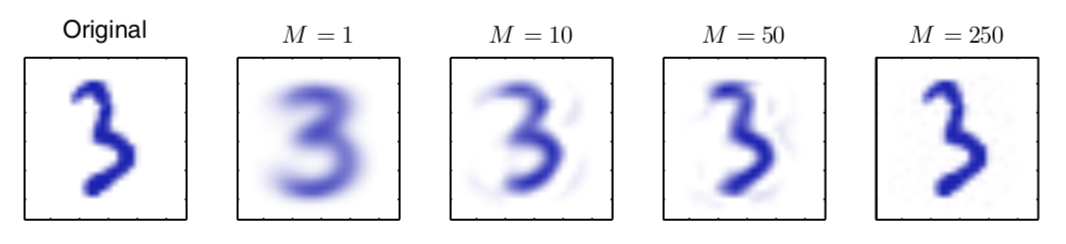
\includegraphics[scale=.6]{images/pca.png}
	\caption{PCA on an image with different number of principal components}
	\label{fig:pca}
\end{figure}

As seen, we can choose to refine the number of attributes that we keep, making the result of our PCA analysis very similar to the original. Such a property is not available in our implementation of the Discrete Fourier Transform. As seen earlier, the DFT automatically retains the frequencies that compose the rest of the image. In addition, the DFT holds the property that it can be easily reverted with the IDFT, something that does not equivalently exist in PCA. While there are image processing techniques that are capable of sharpening an image, they are not an inverse of PCA. The fact that the DFT has an inverse function makes it an extremely valuable transformation when compared to machine learning data reduction algorithms such as PCA.

In short, while the FFT and DFT have more specific prerequisites for the signal, they are more informative and effective in generating composite frequencies. The FFT algorithm is extremely effective in decomposing images quickly as long as they exist on the real space, while the PCA algorithm is effective in breaking down a numeric dataset into fewer, more valuable attributes.

\newpage

\begin{thebibliography}{200}

\bibitem{Bishop} Bishop, C. M. (2016). \emph{Pattern Recognition and Machine} Learning. New York: Springer.

\bibitem{Cormen} Cormen, T. H., Leiserson, C. E., Rivest, R. L., \& Stein, C. (2009). \emph{Introduction to Algorithms}. Cambridge (Massachusetts): The MIT Press.

\bibitem{Discrete} \emph{Discrete Fourier Transform (numpy.fft)}. NumPy v1.16 Manual. \url{https://docs.scipy.org/doc/numpy/reference/routines.fft.html.} Accessed 2 April 2019

\bibitem{Galvao} Galvao, M. (2013, May 14). \emph{Windowing an audio signal}. Computer Music. \url{https://sites.uci.edu/computermusic/2013/05/14/windowing-an-audio-signal/.} Accessed 2 April 2019

\bibitem{Gonzalez} Gonzalez, R. C., \& Woods, R. E. (2008). \emph{Digital Image Processing.} Upper Saddle RIver: Pearson Prentice Hall.

\bibitem{Han} Han, J., \& Kamber, M. (2012). \emph{Data Mining: Concepts and Techniques}. Haryana, India: Elsevier.

\bibitem{Intuition} Intuition, B. (2018, November 14). \emph{Discrete Fourier transform example - numpy.fft}. YouTube. YouTube. \url{https://www.youtube.com/watch?v=R6u5BFOJDh0}. Accessed 2 April 2019

\bibitem{PythonTutorials} PythonTutorials. (2017, September 15). GitHub. \emph{https://github.com/damian-dz/PythonTutorials}. Accessed 2 April 2019

\bibitem{Saff} Saff, E. B., \& Snider, A. D. (2003). \emph{Fundamentals of complex analysis with applications for engineering and science}. Upper Saddle River, NJ: Prentice Hall.

\bibitem{Sundararajan} Sundararajan, D. (2001). \emph{The Discrete Fourier Transform: Theory, Algorithms and Applications}. Singapore: World Scientific.

\bibitem{Tewari} Tewari, P. (2017). \emph{Audio Compression Using Fourier Transform.} International Journal of Science and Research, 1–4. Accessed 1 April 2019

\end{thebibliography}

\end{document}